% This is text associated with the open textbook "Open Electromagnetics"
% See immediately below for author, date
% This work is licensed under the Creative Commons Attribution-ShareAlike 4.0 International License. (CC BY-SA 4.0) 
% To view a copy of the license, visit http://creativecommons.org/licenses/by-sa/4.0/

%ORB TITLE Coulomb's Law
%ORB AUTHOR 0        # S.W. Ellingson, Virginia Tech (ellingson@vt.edu)
%ORB DATE 20180803   # yyyymmdd
%ORB ABSTRACT Coulomb's Law

\label{m0102_Coulombs_Law} % <-- Must match name of this file and module directory name.  Don't mess with this!
\index{Coulomb's law|(}

Consider two charge-bearing particles in free space, identified as ``particle~1'' and ``particle~2'' in Figure~\ref{m0102_fCoulombsLaw}.
Let the charges borne by these particles be $q_1$ and $q_2$, and let $R$  be the distance between them.
If the particles bear charges of the same sign (i.e., if $q_1q_2$ is positive), then the particles repel; otherwise, they attract.
This repulsion or attraction can be quantified as a force experienced by each particle.  
Physical observations reveal that the magnitude of the force is proportional to $q_1q_2$, and inversely proportional to $R^2$.
For particle~2 we find:
%
\begin{equation}
{\bf F} = \hat{\bf R} F_0 \frac{q_1 q_2}{R^2}
\end{equation}
%
where 
$\hat{\bf R}$ is the unit vector pointing from the particle~1 to the particle~2, and
$F_0$ is a constant.  
The value of $F_0$ must have units of inverse permittivity; i.e., 
(F/m)$^{-1}$.
This is most easily seen by dimensional analysis of the above relationship, including the suspected factor:
\begin{equation}
\frac{\mbox{C}\cdot\mbox{C}}{\mbox{F/m}\cdot\mbox{m}^2} 
= \frac{\mbox{C}\cdot\mbox{C}}{\mbox{F}\cdot\mbox{m}} 
= \frac{\mbox{C}\cdot\mbox{C}}{\mbox{C/V}\cdot\mbox{m}}
= \frac{\mbox{C}\cdot\mbox{V}}{\mbox{m}}
= \frac{\mbox{J}}{\mbox{m}}
= \mbox{N}
\nonumber
\end{equation}
%
where we have used the facts that 
1~F $=$ 1~C/V,
1~V $=$ 1~J/C, and
1~N $=$ 1~J/m.
%
This finding suggests that $F_0\propto\epsilon^{-1}$, where $\epsilon$ is the permittivity of the medium in which the particles exist.
Observations confirm that the force is in fact inversely proportional to the permittivity, with an additional factor of $1/4\pi$ (unitless).  
Putting this all together we obtain what is commonly known as \emph{Coulomb's Law}:
%
\begin{equation}
\boxed{
{\bf F} = \hat{\bf R}\frac{q_1 q_2}{4\pi\epsilon R^2}
}
\end{equation} 
%
\begin{figure}
\begin{center}
\pdftooltip{{  % note double braces
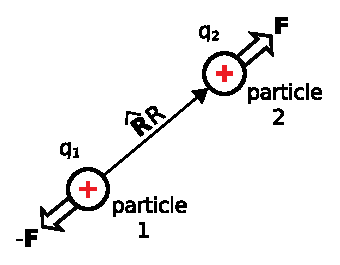
\includegraphics[width=2in]{modules/m0102_fCoulombsLaw.eps}
% https://commons.wikimedia.org/wiki/File:M0102_fCoulombsLaw.svg
}}{The diagram shows two positively-charged particles, particle 1 and particle 2, represented by two circles with red plus signs in the middle. Particle 1 is also labeled q sub 1, and particle 2 is also labeled q sub 2. The distance between them is separated by an arrow pointing from particle 1 to particle 2, labeled bold R-hat * R. An arrow pointing away from particle 1 is labeled -F. An arrow pointing away from particle 2 is labeled F. }
\end{center} 
\centerline{\scriptsize 
\copyright~\hyperref[m0102_fCoulombsLaw_Credit]{K. Kikkeri} 
\href{https://creativecommons.org/licenses/by-sa/4.0/}{CC BY~SA 4.0} 
} 
\caption{
\label{m0102_fCoulombsLaw}
Coulomb's Law describes the force perceived by pairs of charged particles.
}
\end{figure}

Subsequently, the force perceived by particle~2 is equal and opposite; i.e., equal to $-{\bf F}$.
 
Separately, it is known that ${\bf F}$ can be described in terms of the electric field intensity ${\bf E}_1$ associated with particle~1:
%
\begin{equation}
{\bf F} = q_2{\bf E}_1
\end{equation} 
%
This is essentially the \emph{definition} of ${\bf E}_1$, as explained in Section~\ref{m0002_Electric_Field_Intensity}.
Combining this result with Coulomb's Law, we obtain a means to directly calculate the field associated with the first particle in the absence of the second particle:
%
\begin{equation}
\boxed{
{\bf E}_1 = \hat{\bf R}\frac{q_1}{4\pi\epsilon R^2}
}
\label{m0102_eCoulombsLawPointCharge}
\end{equation} 
%
where now $\hat{\bf R}R$ is the vector beginning at the particle~1 and ending at the point to be evaluated.

%--------------------------------
%ORB HIGHLIGHT
\begin{mdframed}[backgroundcolor=yellow!20,nobreak=true] 
The electric field intensity 
\index{electric field intensity}
associated with a point charge (Equation~\ref{m0102_eCoulombsLawPointCharge}) is (1) directed away from positive charge, (2) proportional to the magnitude of the charge, (3) inversely proportional to the permittivity of the medium, and (3) inversely proportional to distance squared. 
\end{mdframed}
%--------------------------------

We have described this result as originating from Coulomb's Law, which is based on physical observations.
However, the same result may be obtained directly from Maxwell's Equations using Gauss' Law (Section~\ref{m0014_Gauss_Law_Integral_Form}).

%--------------------------------
%ORB EXAMPLE
~\\ \begin{example} 
\begin{mdframed}[backgroundcolor=brown!20,linecolor=brown!20]\raggedright
Electric field of a point charge at the origin.
\\~\\
A common starting point in electrostatic analysis is the field associated with a particle bearing charge $q$ at the origin of the coordinate system.
Because the electric field is directed radially away from a positively-charged source particle in all directions, this field is most conveniently described in the spherical coordinate system.
Thus, $\hat{\bf R}$ becomes $\hat{\bf r}$, $R$ becomes $r$, and we have
%
\begin{equation}
{\bf E}({\bf r}) = \hat{\bf r}\frac{q}{4\pi\epsilon r^2}
\end{equation} 

Here's a numerical example. What is the electric field intensity at a distance 1~$\mu$m from a single electron located at the origin, in free space?
In this case, $q\cong -1.60 \times 10^{-19}$~C (don't forget that minus sign!), $\epsilon=\epsilon_0$, $r=1~\mu$m, and we find: 
%
\begin{equation}
{\bf E}({\bf r}) = -\hat{\bf r}\left(1.44~\mbox{kV/m}\right)
\end{equation} 
%
This is large relative to electric field strengths commonly encountered in engineering applications.
The strong electric field of the electron is not readily apparent because electrons in common materials tend to be accompanied by roughly equal amounts of positive charge, such as the protons of atoms.
Sometimes, however, the effect of individual electrons {\it does} become significant in practical electronics through a phenomenon known as \emph{shot noise}.
\index{shot noise}
\end{mdframed}\end{example}
%--------------------------------

{\bf Additional Reading:}
\begin{itemize}
\item ``\href{https://en.wikipedia.org/wiki/Coulomb's_law}{Coulomb's Law}'' on Wikipedia.
\item ``\href{https://en.wikipedia.org/wiki/Shot_noise}{Shot Noise}'' on Wikipedia.
\end{itemize}

\index{Coulomb's law|)}
